% ============================================================================
% The Topology of Reachable Nature  —  PORTABLE (article) build
% Compiles anywhere (pdflatex + bibtex). Shares abstract.tex + body.tex with the
% Springer build (main-springer.tex). For NNJ submission use main-springer.tex
% with the sn-jnl class (see README-springer.md).
% ============================================================================
\documentclass[11pt]{article}

\usepackage[utf8]{inputenc}
\usepackage[T1]{fontenc}
\usepackage{amsmath,amssymb}
\usepackage{booktabs}
\usepackage{graphicx}
\usepackage{geometry}
\geometry{margin=1in}
\usepackage[numbers,sort&compress]{natbib}
\usepackage{hyperref}
\usepackage{xspace}

\newcommand{\Drho}{D(\rho)\xspace}
\newcommand{\rhostar}{\rho^{*}\xspace}

\title{The Topology of Reachable Nature: Persistent Homology and the\\
Resilience of Green-Space Access in Cities of Contrasting Morphology}
\author{Seyda Emekci\\
\small Department of Architecture, Ankara Y{\i}ld{\i}r{\i}m Beyaz{\i}t University}
\date{}

\begin{document}
\maketitle

\begin{abstract}
Sustainable Development Goal~11.7 calls for universal access to green and public
space, yet accessibility is almost always quantified as a static snapshot that
says nothing about how access degrades when the street network is disrupted. We
introduce a \emph{topological resilience metric} for accessibility: the
Wasserstein distance between the persistent-homology diagram of a city's
green-space accessibility field before and after network disruption, traced as a
function of disruption intensity~$\rho$. The area under this degradation curve
and its critical transition $\rho^{*}$ summarise how robustly a place keeps its
population close to nature. Applying the metric to five morphologically
contrasting cities (İstanbul, Barcelona, Amsterdam, Bogotá, Phoenix) at the
level of $2{,}603$ intra-urban districts, we find that street-network morphology
is a strong, statistically significant predictor of green-space access
resilience: in a district-level regression with city fixed effects, street
circuity, orientation entropy, mean segment length and intersection density are
all significant ($p<0.01$; three at $p<10^{-8}$). The relationship is robust: the
three strongest effects keep their sign and significance under both random and
targeted disruption and across district resolutions spanning a $28\times$ range of
unit counts. The signal lives in dimension-0 homology---the merging of well-served
regions---rather than in enclosed ``access deserts,'' a finding that only emerges
on real street networks.

\end{abstract}

\section{Introduction}
Target~11.7 of Sustainable Development Goal~11 commits states to provide
``universal access to safe, inclusive and accessible, green and public spaces''
\citep{un2015sdg}. Planners typically measure progress with catchment or
proximity analyses: the share of residents within a walking threshold of a park.
Such measures are static. They describe access on an ordinary day and are silent
about \emph{resilience}---how access to nature holds up when the pedestrian
network is degraded by a flood, an earthquake, or the closure of a critical
bridge or street. Two gaps follow. First, a city can score well on average
proximity yet collapse under modest disruption; average accessibility does not
reveal this fragility. Second, accessibility work rarely connects the
\emph{shape} of access to urban \emph{form}, which is precisely the
architecture--mathematics question that motivates this collection.

Persistent homology (PH) offers a principled, multi-scale, coordinate-free
language for the ``holes'' and connected pieces of a coverage pattern
\citep{otter2017roadmap,feng2021tda}. PH has been used to detect coverage gaps
for amenities such as polling sites \citep{hickok2022polling} and healthcare
\citep{gonzalez2025healthcare}, to read the topology of urban congestion
\citep{wu2017congestion}, and to quantify displacement under urban expansion
\citep{rodriguez2025displacement}. What is \emph{not} novel is using PH to find
accessibility ``holes'' for an amenity. Our contribution is to move from
\emph{detecting} coverage gaps to \emph{measuring the resilience of the access
topology} and to \emph{linking that resilience to urban form}.

\paragraph{Contributions.}
\begin{itemize}
  \item \textbf{A topological resilience metric} (the mathematics). We define
    $\Drho$, the Wasserstein distance between the persistent-homology diagram of
    the green-space accessibility field before and after disruption of intensity
    $\rho$, and summarise it by an area-under-curve (AUC) and a critical
    transition $\rhostar$ (Section~\ref{sec:method}).
  \item \textbf{First topological treatment of SDG~11.7 green-space access} in an
    architecture--mathematics framing.
  \item \textbf{A district-level morphology$\leftrightarrow$resilience result}
    across $2{,}603$ districts in five cities, with city fixed effects, showing a
    consistent association between street-network morphology and access resilience
    whose sign is stable across disruption models and district resolutions
    (Section~\ref{sec:results}).
\end{itemize}

\section{Related work}
\emph{TDA of spatial systems.} \citet{feng2021tda} survey persistent homology for
spatial data; \citet{otter2017roadmap} give the computational foundations. Within
urban analysis, \citet{wu2017congestion} read traffic congestion as a barcode,
and a line of ``resource coverage'' work applies sublevel or network-distance
filtrations to amenity access: polling places \citep{hickok2022polling} and
sexual-health services \citep{gonzalez2025healthcare}. \citet{rodriguez2025displacement}
use PH to quantify displacement under urban expansion. These studies establish
that PH can \emph{locate} coverage holes. We differ on the object of study: we do
not report where the deserts are, but how the whole access topology
\emph{degrades} under disruption, and we regress that degradation on morphology.

\emph{Accessibility and equity.} A large body of work measures green-space access
as a static field, whether by simple footpath proximity \citep{carthy2020greenspace}
or by catchment methods such as the Gaussian two-step floating catchment area
\citep{sun2023catchment}, often to diagnose inequities in who lives close to nature
\citep{asibey2026equity}. Our accessibility field (Section~\ref{sec:method}) is
built the same way---network walking time to the nearest green space---but is then
read topologically and stress-tested, rather than thresholded once.

\emph{Street-network morphology.} We characterise form with standard descriptors
computed from OpenStreetMap via OSMnx \citep{boeing2017osmnx}: intersection
density, circuity, orientation entropy, and mean street-segment length. Relating
these to a resilience outcome is the architecture--mathematics bridge of this
paper.

\section{Mathematical background}
Let $G=(V,E)$ be the pedestrian network and $f:V\to\mathbb{R}$ a scalar field
giving, at each node, the network walking time to the nearest green-space access
point. The \emph{sublevel-set filtration} of $f$ builds a growing simplicial
complex $K_t = \{\,\sigma : \max_{v\in\sigma} f(v)\le t\,\}$. As the threshold
$t$ (walk-minutes) rises, well-served regions appear and merge. Persistent
homology records, for each topological feature, a birth $b$ and death $d$; the
multiset of points $(b,d)$ is the \emph{persistence diagram} $\mathrm{Dgm}_k(f)$
in homological dimension $k$ \citep{edelsbrunner2000persistence}. Dimension~0
tracks connected components (the merging of well-served regions); dimension~1
tracks loops (enclosed voids, i.e.\ access ``deserts'').

The distance between two diagrams is measured by an optimal matching. The
$1$-Wasserstein distance is
\[
W_1(X,Y)=\min_{\gamma}\sum_{x\in X}\lVert x-\gamma(x)\rVert,
\]
minimised over bijections $\gamma$ between the diagrams (with matching to the
diagonal allowed). Wasserstein and bottleneck distances are stable to
perturbations of $f$ \citep{cohensteiner2007stability}: a small change in the
field produces a small change in the distance. Stability is a mathematical
well-posedness property, not a validation that diagram distance measures
\emph{urban} resilience; we use it only to justify that $\Drho$ responds
continuously and monotonically to progressive network damage, and we treat the
metric throughout as a \emph{proposed proxy} for how the access topology holds up,
to be validated against independent resilience evidence in future work rather than
as ground truth. We compute PH with GUDHI \citep{gudhi} and diagram distances with
\texttt{persim}.

\section{Methodology}\label{sec:method}
\paragraph{Data.} For each city we take the pedestrian network and green/public
spaces from OpenStreetMap via OSMnx \citep{boeing2017osmnx}, and we fix the
analysis extent to the city's \emph{urban centre} polygon from the GHS Urban
Centre Database \citep{ghsl2019ucdb} so that extents are comparable across
countries. Green spaces are the OSM classes \texttt{leisure=park|garden|recreation\_ground},
\texttt{landuse=grass|recreation\_ground}, \texttt{place=square} and
\texttt{natural=wood}; their centroids, snapped to the nearest network node, are
the access points. This is a deliberately inclusive definition: it merges spaces
of very different type, size and usability (a pocket garden, a city square and a
large wood all count equally), and it takes the centroid as a single access point
rather than modelling entrances or area. We treat every green space as an
equivalent point source; distinguishing quality, size, or public/private status
is left to future work (see Limitations).

\paragraph{Accessibility field.} We assign each node its network walking time (at
$4.8$~km/h) to the nearest green-space access point by multi-source Dijkstra,
giving the field $f$ (Fig.~\ref{fig:accessfield}). The field is defined over
\emph{network nodes}, each weighted equally; it is a property of the pedestrian
network's spatial reach to green space, not a population-weighted or
distributional measure. Our metric therefore speaks to one facet of SDG~11.7---the
network's capacity to keep locations close to green and public space, and how that
capacity degrades under disruption---and not to the target's population-coverage or
inclusivity dimensions, which would require census and land-use data we do not use
here.

\begin{figure}[t]\centering
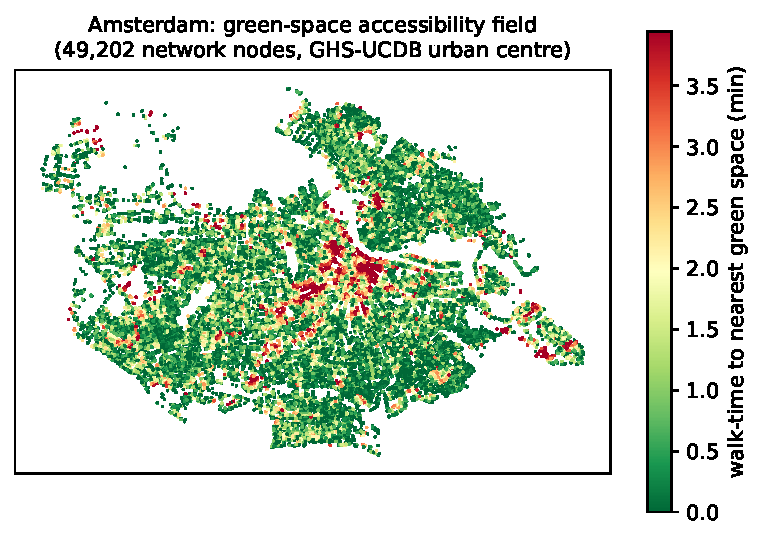
\includegraphics[width=0.72\linewidth]{figures/fig_accessfield.pdf}
\caption{Green-space accessibility field for Amsterdam: each of the $49{,}202$
pedestrian-network nodes inside the GHS-UCDB urban centre, coloured by network
walking time to the nearest green space. Green marks well-served locations,
red the access-poor pockets whose merging structure the resilience metric tracks.}
\label{fig:accessfield}
\end{figure}

\paragraph{Resilience metric.} Let $\mathrm{Dgm}(f)$ be the baseline diagram. A
disruption of intensity $\rho\in[0,1]$ removes a fraction $\rho$ of network
edges; we recompute the field and diagram on the disrupted network and define the
degradation
\[
\Drho=\underset{r}{\mathbb{E}}\;W_1\!\big(\mathrm{Dgm}(f),\,\mathrm{Dgm}(f_{\rho,r})\big),
\]
averaged over $r$ replicate disruptions. We consider three disruption families:
uniformly random edge removal (percolation-style), targeted removal of
high-betweenness edges, and hazard removal of edges in low-elevation zones. Exact
edge betweenness is $O(V\lvert E\rvert)$ and intractable at city scale, so the
targeted scenario ranks edges by betweenness approximated from $k=500$ sampled
pivot sources. The
resilience of a place is summarised by the area under the curve
$\mathrm{AUC}=\int_0^{\rho_{\max}}\Drho\,d\rho$ (normalised by the $\rho$-range)
and the critical transition $\rhostar$, the smallest $\rho$ at which $\Drho$ first
reaches half its maximum---a percolation-style threshold at which access
structure breaks down.

\paragraph{Homology dimension and denoising.} On real street networks the
sublevel filtration's finite $H_1$ is nearly empty: a street graph contains few
triangles, so the network's cycles are never filled and almost all $H_1$ classes
are essential (infinite) and carry no finite persistence. In Amsterdam, for
example, the baseline diagram has $6{,}449$ finite $H_0$ classes but only a single
finite $H_1$ class (Fig.~\ref{fig:persistence}). The resilience signal therefore
lives in \emph{dimension~0}: the merging structure of well-served regions. We
consequently compute $\Drho$ on $H_0$. To keep the exact Wasserstein matching
tractable on city-scale diagrams we apply persistence thresholding, discarding
$H_0$ classes with lifetime below $1$~walk-minute (topological noise); this
preserves the ranking and $\rhostar$ while reducing reported magnitudes by roughly
$10$--$15\%$.

\begin{figure}[t]\centering
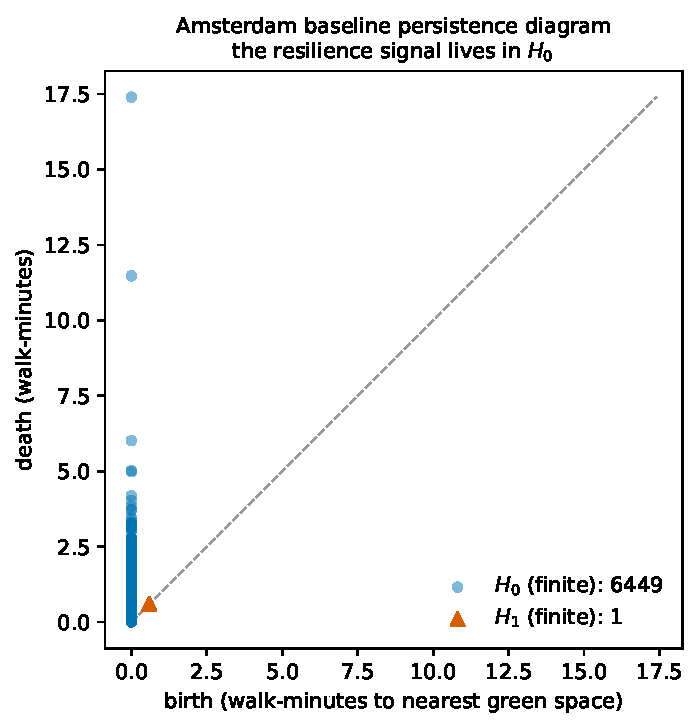
\includegraphics[width=0.55\linewidth]{figures/fig_persistence.pdf}
\caption{Persistence diagram of the Amsterdam baseline accessibility field. The
finite part is carried almost entirely by $H_0$ ($6{,}449$ classes---the merging
of well-served regions as the walk-time threshold rises) with only a single finite
$H_1$ class, motivating an $H_0$-based resilience metric.}
\label{fig:persistence}
\end{figure}

\paragraph{Districts and inference.} Statistical inference rests not on five
cities but on intra-urban \emph{districts}: we tile each urban-centre boundary
with a uniform H3 hexagonal grid (resolution~8, $\approx0.7$~km$^2$ cells) and
compute, per district, its local resilience summaries and its local morphology
(intersection density, circuity, orientation entropy, mean segment length, and a
green-space fragmentation index---the number of distinct green-space patches per
square kilometre of green area within the district, computed on the green space
clipped to each hex so that it varies between districts rather than being a
per-city constant collinear with the fixed effects). We then fit
\[
\mathrm{AUC}_i = \beta^\top \mathbf{m}_i + \alpha_{c(i)} + \varepsilon_i,
\]
an ordinary-least-squares regression of district AUC on morphology
$\mathbf{m}_i$ with \emph{city fixed effects} $\alpha_{c(i)}$ absorbing all
between-city confounds. The five cities serve as a typological overlay, not as
the inferential sample.

\section{Case studies}
We study five cities chosen to span street morphology, planning regime and
Global North/South divide: İstanbul (organic, hilly, polycentric, seismic),
Barcelona (Cerdà grid with superblock interventions), Amsterdam (compact, canal,
walkable), Bogotá (dense informal--formal mix), and Phoenix (low-density grid
sprawl). Boundaries are the GHS-UCDB urban-centre polygons; homonymous centres
(e.g.\ Barcelona, Spain vs.\ Venezuela) are disambiguated by largest true
(equal-area) extent.

\section{Results}\label{sec:results}
The random-disruption analysis yields $2{,}603$ qualifying districts
(Table~\ref{tab:coverage}); only $2.6\%$ have zero AUC. District mean AUC ranks
Amsterdam as the most resilient and İstanbul/Bogotá as the least
(Table~\ref{tab:typology}); Phoenix has the earliest breakdown ($\rhostar=0.16$).
The district-mean ranking and the whole-city ranking below agree at the extremes
(Amsterdam most resilient, Bogotá least) but not in the middle---Barcelona is
mid-ranked by district mean yet most resilient at the whole-city scale---a
reminder that AUC is comparable across cities only in broad ordering, not level.

\begin{table}[t]\centering
\caption{District coverage (H3 resolution~8). Inference rests on $n=2{,}603$.}
\label{tab:coverage}
\begin{tabular}{lccccc c}
\toprule
City & Amsterdam & Barcelona & İstanbul & Bogotá & Phoenix & Total\\
\midrule
Districts & 227 & 147 & 729 & 538 & 962 & \textbf{2{,}603}\\
\bottomrule
\end{tabular}
\end{table}

\begin{table}[t]\centering
\caption{City typology (descriptive). Higher mean AUC $\Rightarrow$ access
topology changes more under disruption $\Rightarrow$ \emph{less} resilient.}
\label{tab:typology}
\begin{tabular}{lccc}
\toprule
City & mean AUC & mean $\rhostar$ & mean $H_0$ total persistence\\
\midrule
Amsterdam & 4.46 & 0.25 & 13.11\\
Phoenix   & 6.68 & 0.16 & 8.08\\
Barcelona & 7.67 & 0.28 & 13.63\\
İstanbul  & 7.75 & 0.20 & 12.84\\
Bogotá    & 8.02 & 0.24 & 16.90\\
\bottomrule
\end{tabular}
\end{table}

The headline result is the district-level regression (Table~\ref{tab:regression}),
fit over the full disruption grid ($8$ intensities $\times\,10$ replicates).
With city fixed effects and $n=2{,}603$, three of five morphology descriptors are
significant, two of them at $p<10^{-15}$. Because the coefficient sign is on AUC
(higher AUC = less resilient), a negative coefficient means the descriptor is
associated with \emph{greater} resilience. More circuitous networks (coef $-10.16$)
and longer street segments ($-0.048$) are associated with more resilient
green-space access, whereas higher orientation entropy ($+1.01$) is associated with
less. Intersection density is negatively signed, consistent with local redundancy
aiding resilience, but is not significant ($p=0.22$), so we treat it as at most
suggestive. Green-space fragmentation is likewise not significant once it varies
within cities and city fixed effects are included. Because districts nest within
five cities, we also report city-clustered standard errors
(Table~\ref{tab:clustered}) and a spatial-autocorrelation diagnostic
(Table~\ref{tab:moran}); we return to their implications in the Limitations.

\begin{table}[t]\centering
\caption{District fixed-effects regression, $\mathrm{AUC}\sim\text{morphology}+C(\text{city})$,
$n=2{,}603$, random-disruption scenario at the full disruption grid
($8\times10$). Classical OLS standard errors; see Table~\ref{tab:clustered} for
city-clustered inference. Sig.: $^{***}p<0.001$.}
\label{tab:regression}
\begin{tabular}{lrrr}
\toprule
Morphology descriptor & coef & std.\ err. & $p$-value\\
\midrule
circuity & $-10.156$ & $1.167$ & $5.5\times10^{-18}$ $^{***}$\\
mean street length & $-0.0476$ & $0.0058$ & $3.7\times10^{-16}$ $^{***}$\\
orientation entropy & $+1.015$ & $0.200$ & $4.4\times10^{-7}$ $^{***}$\\
intersection density & $-0.091$ & $0.074$ & $0.22$\\
green-space fragmentation & $-2.0\times10^{-6}$ & $4.2\times10^{-6}$ & $0.64$\\
\bottomrule
\end{tabular}
\end{table}

\begin{table}[t]\centering
\caption{Sensitivity of the regression inference to how standard errors treat the
nesting of districts within cities. Coefficients are unchanged; only the standard
errors and $p$-values differ. HC3 is heteroskedasticity-robust; the last two
columns cluster by city (five clusters). Circuity and mean street length stay
significant under city clustering; orientation entropy does not.}
\label{tab:clustered}
\begin{tabular}{lrrrr}
\toprule
Morphology descriptor & coef & SE (HC3) & SE (cluster) & $p$ (cluster)\\
\midrule
circuity & $-10.156$ & $1.397$ & $2.946$ & $5.7\times10^{-4}$ $^{***}$\\
mean street length & $-0.0476$ & $0.0066$ & $0.0089$ & $7.7\times10^{-8}$ $^{***}$\\
orientation entropy & $+1.015$ & $0.220$ & $0.894$ & $0.26$\\
intersection density & $-0.091$ & $0.092$ & $0.214$ & $0.67$\\
green-space fragmentation$^{\dagger}$ & $-2.0\times10^{-6}$ & $5.9\times10^{-6}$ & $6.1\times10^{-7}$ & $<10^{-2}$\\
\bottomrule
\end{tabular}

\footnotesize$^{\dagger}$The apparent clustered significance of green-space
fragmentation is a five-cluster artefact of the cluster-robust variance around a
coefficient that is effectively zero ($|\text{coef}|<10^{-5}$); it is not a
substantive effect.
\end{table}

\begin{table}[t]\centering
\caption{Global Moran's~$I$ of the fixed-effects regression residuals within each
city, using first-ring H3 adjacency as the spatial weights ($999$ permutations).
Residuals show weak but significant positive spatial autocorrelation in every city,
motivating an explicit spatial specification in future work.}
\label{tab:moran}
\begin{tabular}{lccc}
\toprule
City & districts & Moran's $I$ & $p$ (perm.)\\
\midrule
Amsterdam & 226 & $0.080$ & $0.031$\\
Barcelona & 147 & $0.178$ & $0.001$\\
Bogotá    & 538 & $0.142$ & $0.001$\\
İstanbul  & 729 & $0.112$ & $0.001$\\
Phoenix   & 962 & $0.058$ & $0.003$\\
\bottomrule
\end{tabular}
\end{table}

\begin{figure}[t]\centering
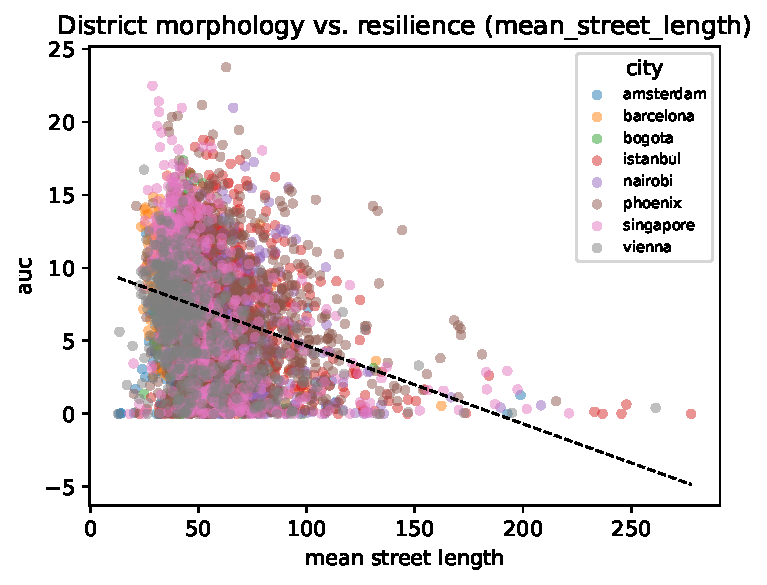
\includegraphics[width=0.72\linewidth]{figures/fig6_morphology.pdf}
\caption{Headline morphology$\leftrightarrow$resilience relationship. Each point
is one of the $2{,}603$ districts, coloured by city; the dashed line is the
pooled least-squares fit. Higher AUC indicates a district whose green-space
access topology degrades more under disruption (less resilient).}
\label{fig:morphology}
\end{figure}

At the whole-city scale (computed on the same UCDB-clipped networks), the
degradation curves $\Drho$ rise smoothly and rank the cities consistently with
the district typology (Fig.~\ref{fig:resilience}). City-level AUC is computed on
the full-city diagram (thousands of $H_0$ classes) and is therefore two to three
orders of magnitude larger than the per-district means of Table~\ref{tab:typology};
only the relative ordering is comparable across the two scales. City-level AUC is
lowest---most resilient---for Barcelona ($620$) and Amsterdam ($898$), and highest
for İstanbul ($2440$) and Bogotá ($2828$), with Phoenix in between ($2053$). The
cities we would informally call compact---Barcelona and Amsterdam---retain more of
their access topology under disruption than the large, sprawling or polycentric
ones; we describe this pattern with the measured morphology descriptors rather
than with ``walkability,'' which we do not model directly. Under
extreme removal ($\rho=0.5$) the İstanbul and Phoenix curves turn down as the
network fragments so heavily that unreachable nodes drop out of the finite
diagram, a signature of near-total collapse rather than of recovered access.

\begin{figure}[t]\centering
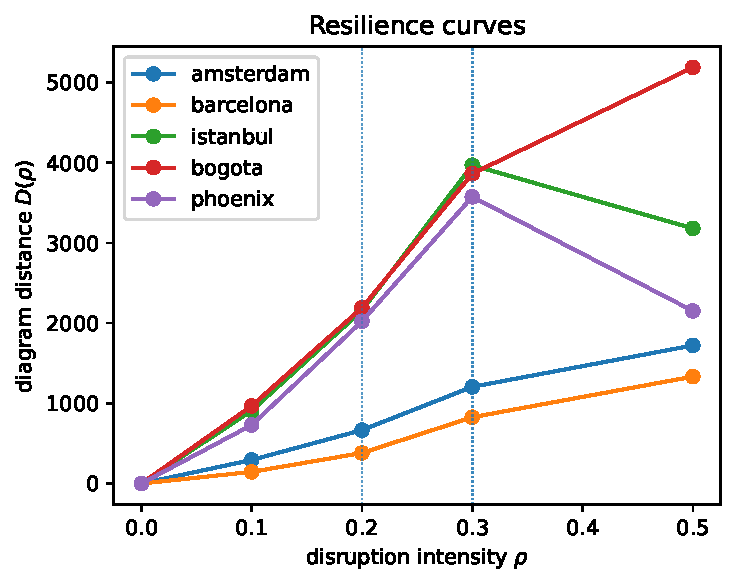
\includegraphics[width=0.72\linewidth]{figures/fig5_resilience.pdf}
\caption{City-level resilience curves $\Drho$ for all five cities (random-disruption
scenario), computed on the UCDB-clipped networks. Dotted vertical lines mark each
city's critical transition $\rhostar$.}
\label{fig:resilience}
\end{figure}

\paragraph{Robustness across disruption scenarios.} Repeating the analysis under
\emph{targeted} disruption (removal of high-betweenness edges, ranked by
$k{=}500$-sampled betweenness) reproduces every coefficient sign in
Table~\ref{tab:regression}. The three descriptors significant under random
disruption stay significant---circuity $-5.77$ ($p=4.6\times10^{-10}$), mean street
length $-0.034$ ($p=2.7\times10^{-13}$), orientation entropy $+0.50$
($p=1.6\times10^{-3}$)---and intersection density, not significant under the full
random grid, reaches $p=0.022$ here ($-0.135$), consistent with our reading of it
as the weakest, grid-sensitive effect; green-space fragmentation is again not
significant. Targeted disruption removes fewer but more critical edges, so absolute
AUC values are lower (e.g.\ Amsterdam mean AUC $2.03$ vs.\ $4.46$ under random), but
the morphology$\leftrightarrow$resilience relationship and the city
ranking are unchanged. The finding is therefore not an artefact of the random
disruption model.

A third, \emph{hazard} scenario (removing edges near the lowest-elevation
$10\%$ of nodes, from AWS Terrain Tiles DEMs) is topography-dependent and much
milder: substantial only in the two flattest cities (Amsterdam and the Phoenix
basin, mean AUC $0.09$ and $0.31$) and near-zero in the hilly or high-altitude
ones (İstanbul, Barcelona, Bogotá; mean AUC $\le0.01$), where the lowest cells
sit at the waterfront and disconnect only a shoreline fringe. This localized
perturbation barely moves the city-wide $H_0$ topology, so it does not resolve a
morphology signal (only orientation entropy remains significant, $+0.10$,
$p=0.01$); we read this as a limitation of the mild, $\rho$-capped low-elevation
proxy rather than a contradiction, and it motivates a stronger flood model that
removes \emph{all} inundated edges.

\paragraph{Disruption-grid sensitivity.} The headline regression uses the full
$8\times10$ disruption grid. A coarser $5\times3$ grid (fewer intensities and
replicates) leaves every coefficient sign unchanged and keeps the three headline
descriptors significant at $p<10^{-3}$ (circuity $-8.99$, mean street length
$-0.0478$---essentially identical to the full grid's $-0.0476$---and orientation
entropy $+1.17$), while the city AUC ranking and $\rhostar$ values agree within
$\approx0.02$. The one descriptor that moves across grids is intersection density:
significant on the coarse grid ($-0.199$, $p=8.6\times10^{-3}$) but not on the full
grid ($p=0.22$). We therefore report the more demanding full grid as the headline
and treat intersection density as the weakest, grid-sensitive effect.

\paragraph{Resolution sensitivity.} Re-running the analysis at H3 resolutions~$7$
(coarse, $485$ districts) and~$9$ (fine, $13{,}782$ districts) leaves the result
unchanged in sign and significance for the three strongest descriptors: circuity,
orientation entropy and mean street length remain significant at $p<10^{-3}$ with
the same signs across all three resolutions, a $28\times$ range of district
counts. Coefficient magnitudes scale with cell size (larger cells yield larger
per-district AUC), but the direction of every effect is stable; only
green-space fragmentation, non-significant throughout, varies.
Figure~\ref{fig:robustness} summarises both robustness axes.

\begin{figure}[t]\centering
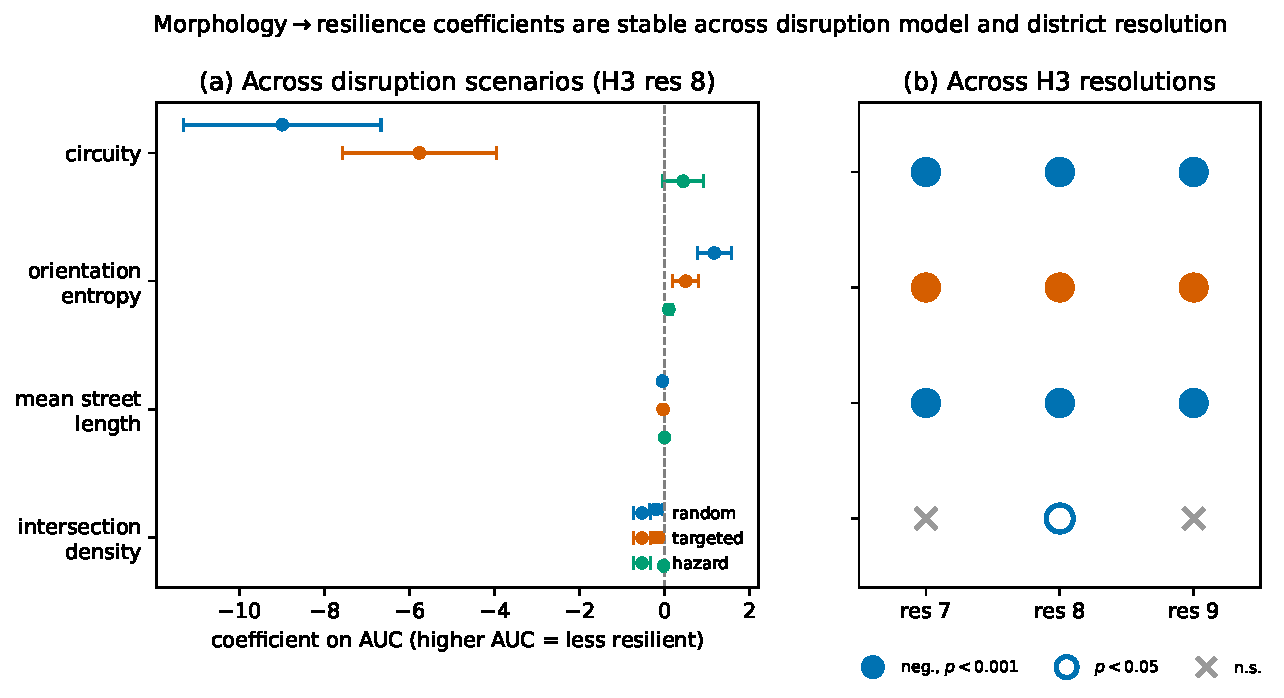
\includegraphics[width=\linewidth]{figures/fig_robustness.pdf}
\caption{Robustness of the morphology$\leftrightarrow$resilience relationship.
\textbf{(a)} Regression coefficients (with $95\%$ confidence intervals) for each
morphology descriptor under the three disruption scenarios at H3 resolution~8;
the coefficient signs agree across scenarios, and the three headline descriptors
(circuity, mean street length, orientation entropy) stay significant, while
intersection density crosses zero under random disruption. \textbf{(b)} Sign and
significance of each coefficient across H3 resolutions $7$/$8$/$9$: the three
headline descriptors stay significant with a constant sign, while intersection
density---the weakest, grid-sensitive effect---is not significant at the headline
full-grid specification.}
\label{fig:robustness}
\end{figure}

\section{Discussion}
The results give an interpretable, architecture-facing reading of resilience.
The robust effects are circuity and segment length: districts with more circuitous
routing and longer segments retain more of their well-served structure when edges
are removed, because alternative paths to green space survive the loss of any one
link. Denser intersections point the same way (locally redundant networks should
be more resilient) but the effect is not statistically robust here, so we do not
lean on it. Districts with more disordered street orientation (higher entropy) are
more brittle. That the signal That the signal
is carried by $H_0$ rather than $H_1$ has a concrete planning meaning. In
green-dense cities the structure that matters is not isolated ``deserts''
surrounded by served land but the connectivity of the served regions themselves,
and that connectivity is what disruption erodes.

\paragraph{Limitations.} We group the caveats by the kind of claim they qualify.

\emph{Inference and spatial dependence.} The design is cross-sectional and
observational, so the regression identifies \emph{associations} between morphology
and topological resilience, not causal effects. Districts are also not independent:
they nest within five cities and are spatially contiguous. City fixed effects
absorb between-city confounds, but two residual problems remain. First, the $2{,}603$
districts furnish only five clusters for cross-city inference; clustering the
standard errors by city (the level at which disruption is applied) widens the
intervals substantially (Table~\ref{tab:clustered}). Under this conservative
treatment the two strongest effects---circuity ($p=6\times10^{-4}$) and mean
street length ($p=8\times10^{-8}$)---remain significant, but orientation entropy,
significant at the district level, does not ($p=0.26$); with only five clusters
even cluster-robust inference is underpowered, so the classical $p$-values in
Table~\ref{tab:regression} understate uncertainty and are best read as
within-sample descriptive strength rather than as a precise cross-city
significance claim.
Second, the residuals retain weak but statistically significant positive spatial
autocorrelation within \emph{every} city (global Moran's~$I$ on the first-ring H3
adjacency runs from $0.06$ in Phoenix to $0.18$ in Barcelona, all with permutation
$p\le0.03$; Table~\ref{tab:moran}), so an explicit spatial-error or spatial-lag
specification, and richer geographic replication beyond five cities, are natural
next steps.

\emph{Omitted variables.} Morphology is only one of many district attributes that
could drive resilience. Population and built density, land-use mix, total
green-space area and park size, slope, socioeconomic status and pedestrian-network
quality are all uncontrolled; city fixed effects remove their between-city
component but not their within-city variation, so the coefficients may absorb
correlated omitted factors.

\emph{What the metric measures.} $\Drho$ is a \emph{proposed proxy}: diagram
stability makes it well-posed, but it has not been validated against independent
resilience outcomes (observed service loss after real disruptions). AUC depends on
network and district size and on the number of $H_0$ classes, so it is comparable
across cities only in relative ranking, not in absolute level; $\rhostar$ likewise
depends on the chosen disruption range. The down-turn of the İstanbul and Phoenix
curves at $\rho=0.5$ reflects finite nodes dropping out of the diagram under
near-total fragmentation, not recovered access, and marks the upper edge of the
metric's useful range. Green spaces are treated as equivalent point sources,
ignoring size, quality and public/private status.

\emph{Disruption and data.} Random removal is spatially uniform and does not
reproduce the clustered failures of a real flood or earthquake; targeted removal
addresses criticality but not spatial correlation, and the hazard scenario, a
$\rho$-capped low-elevation proxy, is too mild and topography-dependent to test the
morphology signal and should be replaced by a full flood-zone edge removal.
Targeted betweenness is approximated from $k{=}500$ sampled pivots, as exact
$O(V\lvert E\rvert)$ betweenness is intractable at city scale. Results use a
persistence-thresholded $H_0$ metric, so reported magnitudes are denoised
estimates, though the full disruption grid confirms the coefficient signs,
the significance of the three strongest descriptors, the ranking and $\rhostar$.
OSM completeness varies by city and is not quantified here, and the
network-distance Vietoris--Rips variant of the filtration is left to future work.

Read together, these caveats narrow the claim: within these five cities, and under
synthetic edge-removal disruption, street-network morphology is a consistent
descriptive correlate of green-space access resilience---robust in sign across
disruption models and district resolutions---rather than a causally identified or
cross-city-generalisable driver.

\section{Conclusion}
We defined a topological resilience metric for green-space accessibility---the
Wasserstein degradation curve of persistent-homology diagrams under network
disruption---and showed, across $2{,}603$ districts in five contrasting cities,
that street-network morphology is associated with how robustly a city's
pedestrian network keeps its \emph{locations} close to nature. The association is
consistent rather than proven causal: random and targeted disruption agree on
every coefficient sign, and the signs are stable across H3 district resolutions
spanning a $28\times$ range of unit counts, but the study is cross-sectional and
rests on five cities (see Limitations). The mathematics of persistence turns a
static SDG~11.7 indicator into a dynamic, form-aware one. Future work will
strengthen the hazard model to a full flood-zone removal and add a network-metric
Vietoris--Rips filtration, toward a resilience-aware accessibility standard for
sustainable cities.

\paragraph{Reproducibility.} All data are open (OpenStreetMap, GHS-UCDB) and the
pipeline is open-source Python (OSMnx, NetworkX, GeoPandas, GUDHI/\texttt{persim},
H3, \texttt{statsmodels}); every reported number is recorded in the project's
results log and traces to a committed artifact.


\section*{Declarations}

\paragraph{Funding.} The author received no specific funding for this work.

\paragraph{Competing interests.} The author declares no competing interests.

\paragraph{Data availability.} All input data are open and publicly available.
Pedestrian networks and green/public spaces were obtained from OpenStreetMap via
OSMnx; urban-centre boundaries from the GHS Urban Centre Database (GHS-UCDB
R2019A, European Commission Joint Research Centre); and elevation data from the
public AWS Terrain Tiles service. No new data were collected. The derived
artifacts underlying every reported figure and table (per-district resilience and
morphology tables, regression outputs, and city-level resilience curves) are
recorded in the project's results log, released with the code at
\url{https://github.com/navigaai/nnj-sdg11-topology}.

\paragraph{Code availability.} The complete analysis pipeline is implemented in
open-source Python (OSMnx, NetworkX, GeoPandas, GUDHI, \texttt{persim}, H3,
\texttt{statsmodels}) and is publicly available at
\url{https://github.com/navigaai/nnj-sdg11-topology}, together with the
configuration files and the results log that reproduce every reported number.

\paragraph{Author contributions.} S.\ Emekci (ORCID 0000-0002-5470-6485) conceived
the study, developed the method and software, performed the analysis, and wrote
the manuscript.


\bibliographystyle{plainnat}
\bibliography{references}

\end{document}
